\section{Daten}
\subsection{Stichproben und Merkmale}
\begin{wrapfigure}[12]{r}{0.2\textwidth}
    \centering
    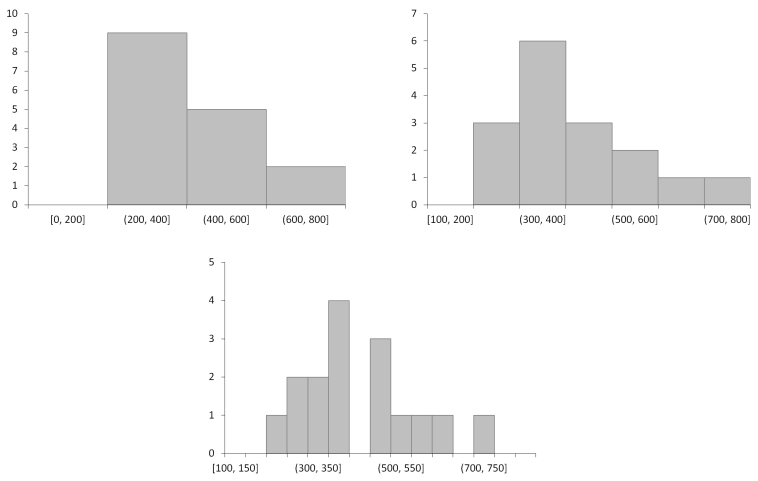
\includegraphics[width=0.2\textwidth]{images/2.2_histogramme.png}
    \caption{Verteilungen mit unterschieldichen \emph{Partitionen}}
    \label{fig:histogramme-binning}
    
\end{wrapfigure}
Elemente einer Stichprobe b(z. B. Umfrageteilnehmer) werden als statische \hl{Einheiten} oder \hl{Merkmalsträger} bezeichnet.
Die von ihnen erhobenen Daten bezeichnet man als \hl{Merkmale} oder \hl{Variablen} (z.b. Geschlecht, Alter, Monatliches Einkommen...). 
Man unterscheidet hierbei zwischen \hl{Zielgrößen} die von anderen Variablen abhängen, \hl{Einflußgrößen} bzw. \hl{Faktoren}, die beobachtet werden können und \hl{Störgrößen, die als latente Größen nicht beobachtbar sind}.
\subsection{Merkmalstypen}
Ein Merkmal heißt \hl{diskret} wenn es nur \emph{endlich} oder \emph{abzählbar} undendlich viele mögliche Ausprägungen besitzt (z. B. Anzahl Personen in einer Wohneinheit). Merkmale, die \emph{überabzählbar} viel Werte annehmen können werden als \hl{stetig}  bezeichnet (z. B. ein Messwert wie Temperatur). Aufgrund von Messungenauigkeiten und/oder Rundungen können \emph{stetige} Werte \emph{diskret} werden. Man spricht von \hl{quasi-stetigen} Werten. 
\\\\
Merkmale lassen sich auch bzglch der \hl{Skalen} unterscheiden, auf denen ihre Ausprägung gemessen werden. \hl{Nominalskala}: Die Ausprägungen entsprechen Namen oder Kategorien, beispielsweise das Geschlecht oder der Typ der Unterkunft. \hl{Ordinalskala}: Ausprägungen besitzten eine natürliche \emph{Ordnung}, \emph{ohne} dass
die Abstände interpretierbar sind. Dies gilt besipielsweise bei Wohnungen für die Entfernung zum Campus oder Notenstufen (-> Rechnungen ergeben keinen sinn). 
\hl{Kardinalskala}: Ausprägungen sind Zahlen, sodass auch die Abstände im Kontext von Differenzen oder Quotientenbildung interpretierbar sind (z. B. Miete, Quadratmeter -> Miete pro Quadratmeter).
Man kann durch Datentransformation von einer feineren auf eine skala mit geringeren Informationsgehalt wechseln (Bsp Gruppierung von Entfernungen zum Campus: 3km, 5km, 10km etc.).
\\\\
Ein Merkmal heißt \hl{qualitativ} oder \hl{kategorial}, wenn es nur endlich viele Ausprägung besitz und diese höchstens \emph{ordinal} skaliert sind.
Anderenfalls ist ein Merkmal \hl{quantitativ}.
\section{Univariante Datenanalyse}
Univariante Daten $\rightarrow$ Merkmale werden als unabhängig angenommen und für einzeln ausgewertet. Häufigkeiten. Stichprobe besteht aus n statistischen Einheiten und $x_1, ..., x_n$ bezeichnet die \emph{beobacheteten} Ausprägungen eines Merkmals $X$. $a_1, ..., a_k$ bezeichnet die Menge der \emph{unterschiedlichen} Ausprägungen, die in der Stichprobe beobachetet wurden.
Die \hl{absolute Häufigkeit} $h(a_j) = h_j$ bezeichnet nun die Anzahl an Beobachtungen des jeweiligen Merkmals $a_j$. \hl{$h(a_i) = h_j := \sum^{n}_{i=1}\mathds{1}(x_i)$} ($\mathds{1}(x_i)$ $\rightarrow$ Indikatorfunktion $\rightarrow$ wenn $a_j == x_i 1$ sonst $0$). \hl{Relative Häufigkeit} ist die absolute Häufigkeit bezogen auf die Größe der Stichprobe \hl{$f(a_j) = f_j := \frac{h_j}{n}$} 
\begin{wrapfigure}{l}{0.2\textwidth}
    \centering
    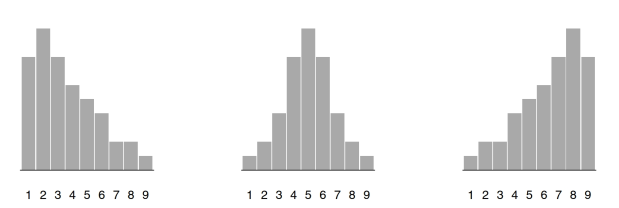
\includegraphics[width=0.2\textwidth]{images/2.3_histogramme_schiefheit.png}
    \caption{linkssteile/rechtsschiefe (links), symmetrische (Mitte) und rechtssteile/linksschiefe
    (rechts) Verteilungen}
    \vspace{-12mm}
    \label{fig:schiefheit}
\end{wrapfigure}
Hat ein Histogramm wie in \cref{fig:schiefheit} einen klaren Höhepunkt spricht man von einer \hl{unimodalen} Verteilung, bei zwei von einer \hl{bimodalen}- und bei mehr als zwei Höhepunkten von einer \hl{multimodalen} Verteilung. Auch wird normalerweise die \hl{Steilheit} benannt (\cref{fig:schiefheit}).
Die \hl{Kummulierte Häufigkeitsverteilung} \hl{$H(x):=\sum^{n}_{i=1}\mathds{1}_{\{x_i \leq x\}} = \underset{j:a_j\leq x}{\sum}h(a_j)$}gibt an, wie viele der Beobachtungen $x_1, ..., x_n$ kleiner oder gleich x sind und analog ergibt sich die \hl{empirische Verteilungsfunktion} \hl{$F(x) := \frac{H(x)}{n} = \frac{1}{n}\sum^{n}_{i=1}\mathds{1}_{\{x_i \leq x\}} = \underset{j:a_j\leq x}{\sum}f(a_j)$} durch die Normierung von $H(x)$ auf die Grundgesamtheit der Stichprobe. \todo[]{evtl. 2.4?} Kumulierte Häufigkeitsverteilungen sind monoton wachsende und rechtsseitig stetige Treppenfunktio-
nen, mit Treppenstufen bei jeder Ausprägung $a_j$ und in der Höhe $h_j$ bzw. $f_j$. Bsp. \glqq Wie häufig leben \emph{höchstens} 3 Personen zusammen?\grqq $\rightarrow$ $F(3) = 3/4$  \glqq Wie häufig leben \emph{mindestens} 2 Personen zusammen?\grqq $\rightarrow$ $1 - F(1) = \frac{13}{16}$ (Werte für F aus Verteilung/Tabelle berechenbar oder aus Diagram ablesbar).
\\\\ 
\emph{Lagemaße}. Das \hl{arithmetisches Mittel} $\bar{x} := \sum^n_{i=1}$ ist zwar anschaulich leicht verständlich, jedoch sehr anfällig gegenüber Ausreißern. Ein stabileres Lagemaß ist der \hl{Median}. Er ist dadurch charakterisiert, dass (mindestens) die Hälfte der Daten größer oder gleich und (mindestens) die Hälfte der Daten kleiner oder gleich seinem Wert ist. \hl{$x_{med} = \begin{cases} x_{(\frac{n+1}{2})} & \text{,falls }n \text{ ungerade} \\
\frac{1}{2}(x_{(\frac{n}{2})} + x_{(\frac{n+1}{2})}) & \text{,falls }n \text{ gerade}
\end{cases}$.} Der \hl{Modus} \hl{$x_{mod} := \underset{a_j}{\text{arg }\text{max }}h(a_j) =\underset{a_j}{\text{arg }\text{max }}f(a_j)$} entspricht dem Element, dass am häufigsten in einer Verteilung auftritt. Für die drei Lagemaße gilt: \emph{Symmetrische Verteilung}: $\bar{x}=x_{med}=x_{mod}$. \emph{Linkssteile/rechtsschiefe Verteilung}: $\bar{x} > x_{med} > x_{mod}$. \emph{Rechtssteile/linksschiefe Verteilung}: $\bar{x}<x_{med}<x_{mod}$
\section{Multivariate Datenanalyse}